% ==========================================
% Section 6: False Predictors (Slides 21-23)
% ==========================================

% Slide 21: False Predictors
\begin{frame}{متغیرهای پیش‌بینی‌کننده کاذب (\lr{False Predictors})}
\begin{columns}[c]
  \begin{column}{0.58\textwidth}
    \begin{itemize}
      \item \textbf{صحت نزدیک به \lr{\textasciitilde 100\%} یک نتیجه عالی است...}
      \begin{itemize}
        \item ...اما نتیجه‌ای است که باید شما را کاملاً به شک بیندازد!
      \end{itemize}
      \vspace{0.3cm}
      \item \textbf{روایتی واقعی از یک تجربه:}
      \begin{itemize}
        \item کار با افزونه داده‌های پیوندی باز (\lr{Linked Open Data - LOD})
        \item تلاش برای پیش‌بینی رتبه‌بندی دانشگاه‌های جهان با داده‌های \lr{DBpedia}
        \item هدف: درک عواملی که یک دانشگاه را به یک دانشگاه برتر (\lr{Top University}) تبدیل می‌کند.
      \end{itemize}
    \end{itemize}
  \end{column}
  \begin{column}{0.40\textwidth}
    \centering
    
\includegraphics[width=\textwidth]{images/page_21_img_1.png}
  \end{column}
\end{columns}
\end{frame}

% Slide 22: The LOD Extension & Leakage
\begin{frame}{متغیرهای پیش‌بینی‌کننده کاذب (\lr{False Predictors})}
\begin{columns}[c]
  \begin{column}{0.58\textwidth}
    \begin{itemize}
      \item \textbf{افزونه داده‌های پیوندی باز (\lr{LOD})}
      \begin{itemize}
        \item استخراج خودکار ویژگی‌های تکمیلی از گراف‌های دانش عمومی (مانند \lr{DBpedia})
        \item بدون نظارت (ویژگی‌ها کاملاً خودکار ایجاد شدند)
      \end{itemize}
      \vspace{0.2cm}
      \item \textbf{مدل آموخته‌شده:}
      \begin{itemize}
        \item \lr{THE < 20 $\to$ TOP = true}
        \item پیش‌بینی‌کننده کاذب: متغیر هدف در میان ویژگی‌ها گنجانده شده بود!
      \end{itemize}
      \vspace{0.2cm}
      \item \textbf{نمونه‌های دیگر:}
      \begin{itemize}
        \item \lr{Mark < 5 $\to$ passed = true}
        \item \lr{Sales > 1000000 $\to$ bestseller = true}
      \end{itemize}
    \end{itemize}
  \end{column}
  \begin{column}{0.40\textwidth}
    \centering
    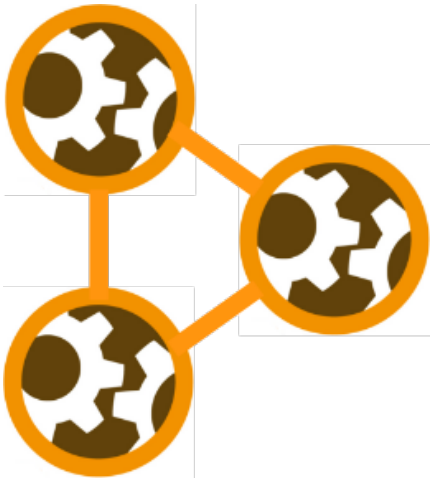
\includegraphics[width=\textwidth]{images/page_22_img_1.png}
  \end{column}
\end{columns}
\end{frame}

% Slide 23: Recognizing False Predictors
\begin{frame}{شناسایی متغیرهای پیش‌بینی کاذب}
\begin{columns}[c]
  \begin{column}{0.55\textwidth}
    \begin{itemize}
      \item \textbf{تحلیل ساختار مدل‌های آموزش‌دیده:}
      \begin{itemize}
        \item مجموعه‌های قاعده که تنها از یک قاعده تشکیل شده‌اند.
        \item درخت‌های تصمیمی که تنها یک گره تصمیم‌گیری دارند.
      \end{itemize}
      \vspace{0.2cm}
      \item \textbf{فرآیند رفع عیب:}
      \begin{itemize}
        \item شناسایی متغیر کاذب با بررسی وزن‌ها یا ریشه درخت
        \item حذف ویژگی کاذب از مجموعه داده
        \item تکرار فرآیند آموزش و ارزیابی
      \end{itemize}
    \end{itemize}
  \end{column}
  \begin{column}{0.43\textwidth}
    \centering
    
\includegraphics[width=\textwidth]{images/page_23_img_1.png}\\[8pt]
    
\includegraphics[width=0.85\textwidth]{images/page_23_img_2.png}
  \end{column}
\end{columns}
\end{frame}
